This section provides the reader with an overview of the ARGOOSE product. The primary operational aspects of the product, from the perspective of end users, maintainers and administrators, are defined here. The key features and functions found in the product, as well as critical user interactions and user interfaces are described in detail.

\subsection{Features \& Functions}
Product shall be expected to detect at least some commercial level drones.  There is no guarantee of detection in military level drones, nor is there any guarantee that all commercial level drones will be detected.  The main detection method is the mode of flight, with spinning rotor being the most ideal--relying on acoustic sensors. The system shall comprise of at least two sub-systems: a drone-detecting edge device and a web-application.  Breaking down the system into two helps with remote access for the customer, than let's say a physical alarm system that sounds off. It also introduces the possibility of scaling the system up (ie. making a network of drone detecting devices).  The hardware components of the system will contain a raspberry pi connected to a GPS, battery and audio sensor system. The audio sensor consists of six microphones aligned in a circular pattern.  In terms of external elements, internet will be utilized, GPS information will be assessed and used, and our web application is an external web server.

\subsection{External Inputs \& Outputs}
\begin{table}[h]
\centering
\begin{tabularx}{\linewidth}{|l|l|>{\raggedright\arraybackslash}X|}
    \hline
\textbf{Name} & \textbf{Description} & \textbf{Use} \\ \hline
Drone & Environmental source of sensory data & Processed for detection \\ \hline
Six-sensor Array & Processed analog audio & Converts analog to digital for system \\ \hline
ODAS & Takes digital signal input & Runs algorithm to detect source of sounds \\ \hline
Secondary Detection System & Self-contained detection & Verify false positives \\ \hline
Drone ID Algorithm & Takes all system input & Decides whether or not something is a drone \\ \hline
GUI & Outputs data in graphical form & notifies users on drone activity \\ \hline
\end{tabularx}
    \end{table}

\subsection{Product Interfaces}
Web application UI shall be readable to an acceptable degree.  The web application doesn't need to be well designed or aesthetically pleasing; however, it needs to at least be readable and understandable for customers and developers.
\begin{figure}[h!]
	\centering
   	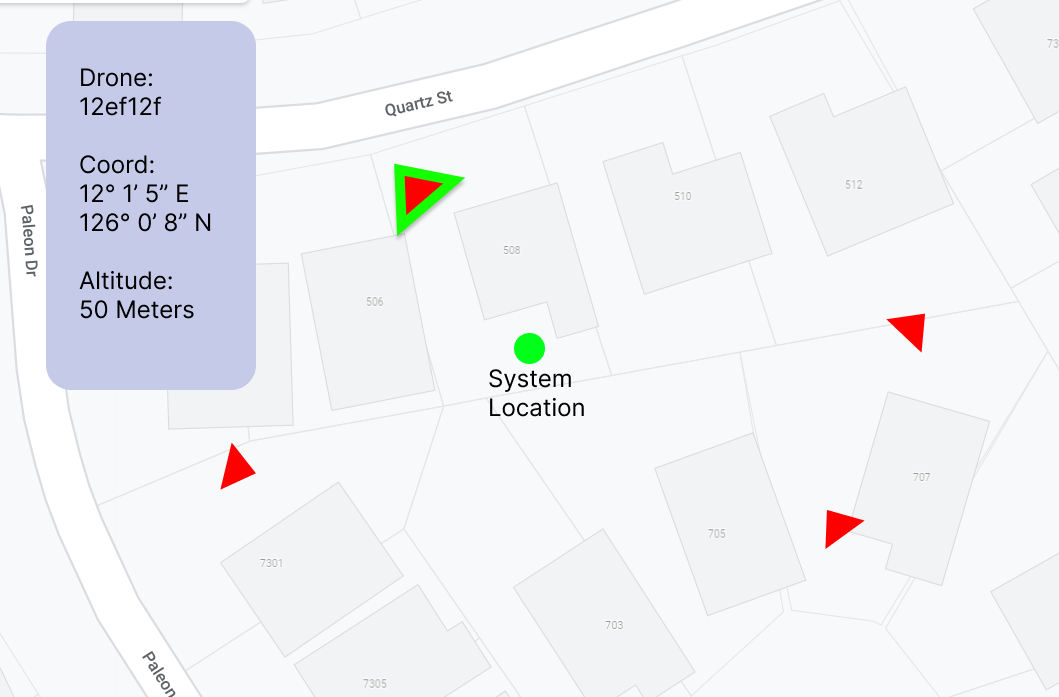
\includegraphics[width=0.60\textwidth]{images/Group 1.png}
   	\caption{Main Detection Page Mock Up}
\end{figure}
